\chapter{Résultats et interprétations}

La perception sonore humaine est dite binaurale : c'est à dire qu'il y a deux «capteurs» (en l'occurence de chaque côté
de la tête).
Cette particularité est importante dans la perception de l'espace, en effet le volume de la tête retarde la propagation
du son tout en déformant celui-ci permettant ainsi un repérage dans le plan horizontal (avec une précsion pouvant aller
jusqu'a un degré~\cite{Vor08}). Le torse a lui aussi une influence, particulièrement pour le répérage dans le plan
vertical. Au cours des mesures pour ce projet, une tête artificielle (sans torse) a été utilisé, le repérage vertical
sera donc difficile à reproduire d'après nos mesures.

\section{Essai 1 : une chanson en salle Mersenne} % {{{1

Le premier essai approfondi est réalisé en salle Mersenne. La source est au point \textbf{Source} (voir
figure~\ref{plan_mersenne}) et le recepteur au point \textbf{P1} (la tête dans la position par défaut).

\subsection{Comparaison perceptive} % {{{2

A l'écoute, la différence entre les deux résultats (monaural et binaural) est flagrante. Alors que la position de la
source est strictement indéterminable en monaural, elle est bien identifiable en binaural.

Des mesures plus précises auraient probablement permis une meilleurs reconnaissance de la géométrie de la salle et des
obstacles, en particulier la paillasse présente sur la droite du récepteur.

\subsection{Comparaison fréquentielle} % {{{2

On note par ailleurs la différence de contenu fréquentiel (et en particulier la différence de niveau) sur la
figure~\ref{comp_mon_min_zoom_150_175}. Cette différence observée sur les spectres est bel et bien en accord avec la
comparaison perceptive menée ci-avant.


\begin{figure}[h!]
    \centering{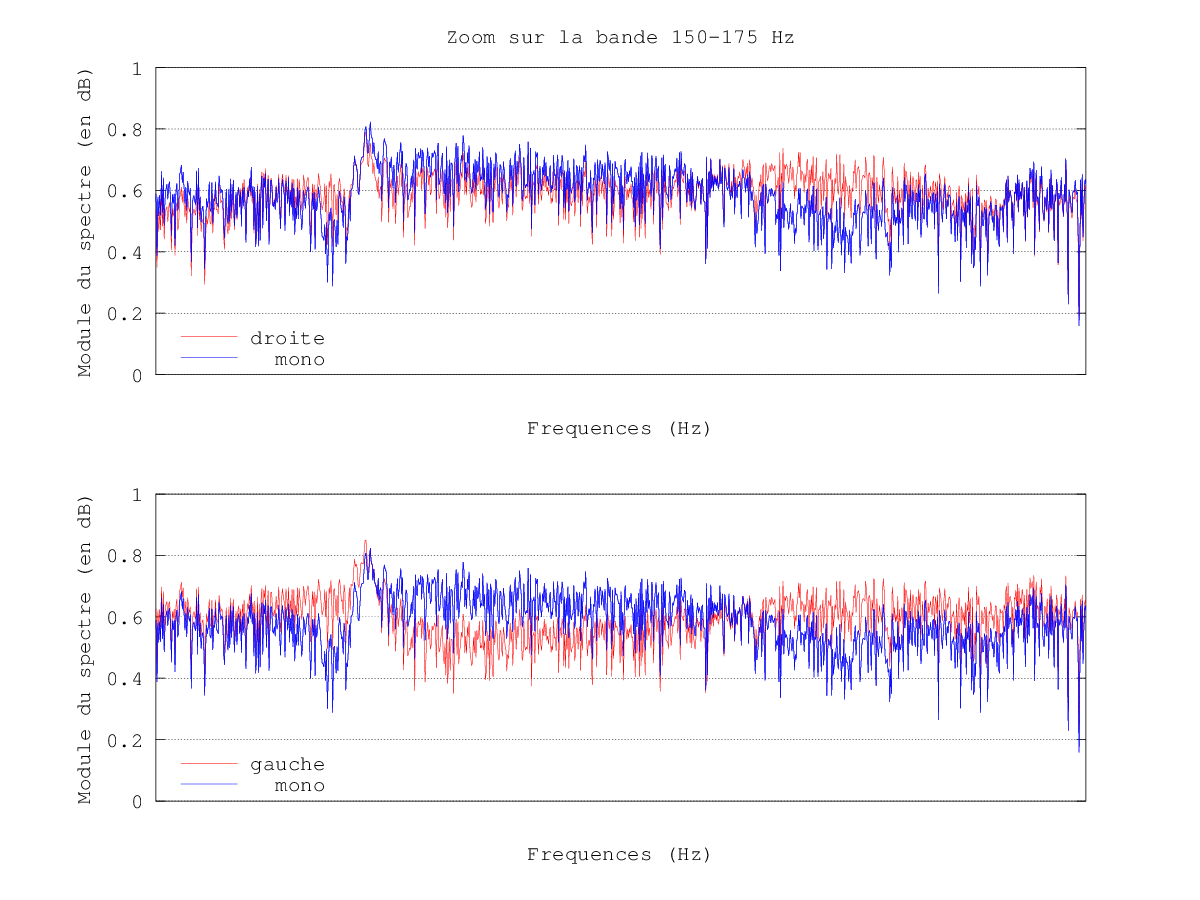
\includegraphics[width=13cm]{comp_mon_min_zoom_150_175.png}}
	\caption{\label{comp_mon_min_zoom_150_175}Comparaison entre les contenus fréquentiels des signaux monaural et
	binaural dans la bande 150-175Hz. On remarque que le signal monaural vient effectivement s'intercaler entre les
	2 canaux du signal binaural (en haut monaural et canal droit, en bas monaural et canal gauche). Une représentation
pleine échelle est disponible en annexe}
\end{figure}

\subsection{Comparaison temporelle} % {{{2 


\begin{figure}[h!]
    \centering{\includegraphics[width=13cm]{comp_mon_bin_P1_enveloppe.png}}
    \caption{\label{comp_mon_bin_P1_enveloppe}}Tracés temporels des signaux convolués pour une RI monaurale (en bleu) et
    une RI binaurale en rouge. En haut pour l'oreille gauche et en bas pour l'oreille droite.}
\end{figure}

La figure~\ref{comp_mon_bin_P1_enveloppe} montre les tracés temporels des signaux convolués en monaural et binaural.
Les différences sont assez minimes (mise à part l'amplitude). Les enveloppes sont très ressemblantes. Un même son est
convolué à chaque fois, le résultat est donc censé être ressemblant.

\section{Essai 2 : Des claquements de mains en salle réverbérante} % {{{1

Un autre essai est mené en salle réverbérante. Il s'agit cette fois de vérifier que les différentes réflexions sont
correctement restituées lors de la convolution.

\subsection{Comparaison temporelle} % {{{2

\begin{figure}[h!]
    \centering{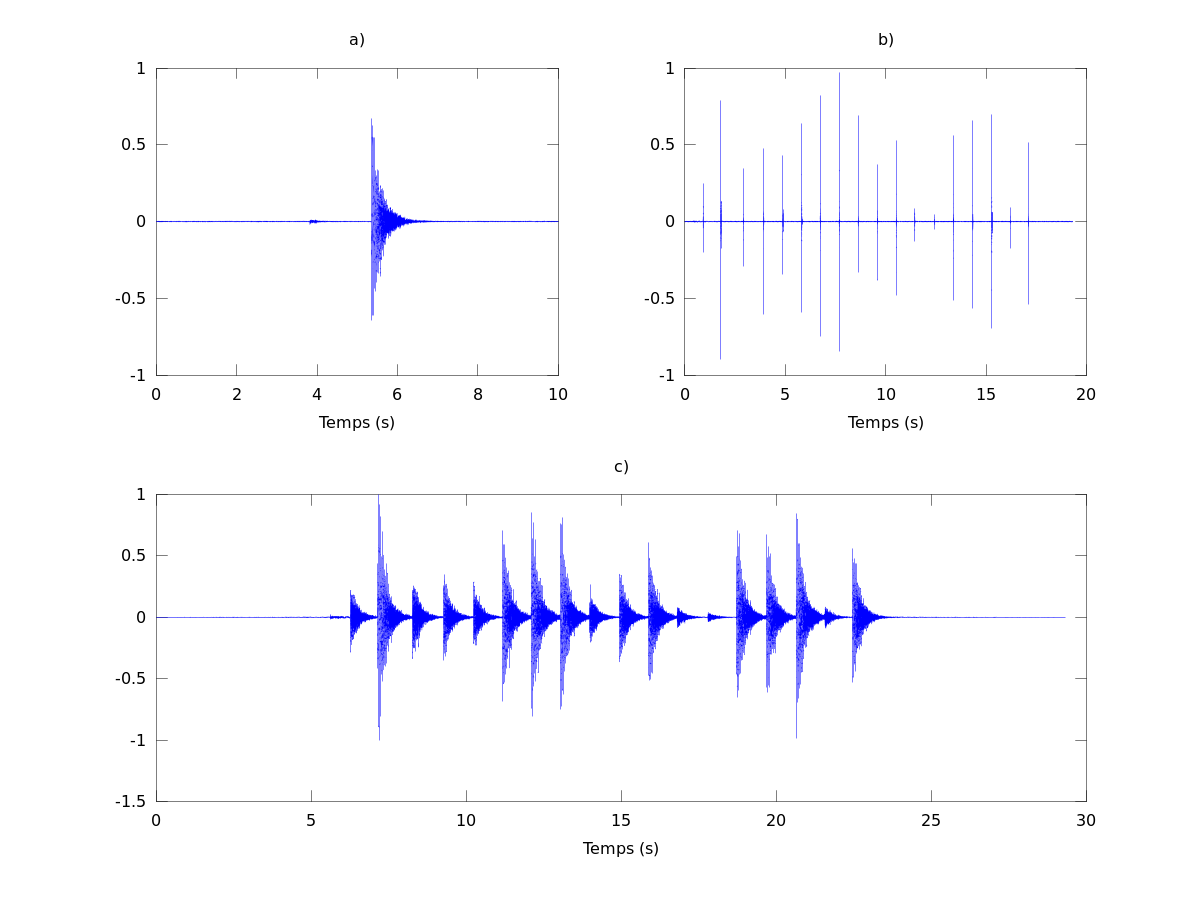
\includegraphics[width=13cm]{temporel_reverb.png}}
	\caption{\label{}Comparaison entre les contenus fréquentiels des signaux monaural et
	binaural dans la bande 150-175Hz. On remarque que le signal monaural vient effectivement s'intercaler entre les
	2 canaux du signal binaural (en haut monaural et canal droit, en bas monaural et canal gauche). Une représentation
pleine échelle est disponible en annexe}
\end{figure}



